\documentclass[tikz,border=2pt]{standalone}
\usepackage{amsmath,amssymb}
\usepackage{xcolor}
\usetikzlibrary{positioning}
\begin{document}
% Extracted from namuenofull.inc; source column: \footnotesize \cite{NU}$_{\rm p{ 164 }}$ II$^*$-IV-$\alpha$
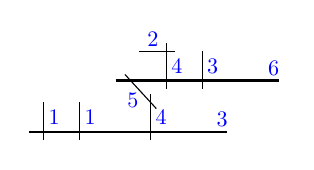
\begin{tikzpicture}[xscale=0.57,yscale=0.62]
\draw[thick,shorten >=2] (-1/3,0)--(253/60,0) node[inner sep=2pt,blue,above left,scale=0.8] {3} node[inner sep=2pt,below left,scale=0.8] {};
\draw[shorten <=-3pt] (0,0)--node[inner sep=2pt,scale=0.8,blue,right] {1} (0,3/5);
\draw[shorten <=-3pt] (4/5,0)--node[inner sep=2pt,scale=0.8,blue,right] {1} (4/5,3/5);
\draw[shorten <=-3pt, shorten >=-3pt] (143/60,0)--node[inner sep=2pt,scale=0.8,blue,right] {4} (143/60,3/5);
\draw[shorten <=-3pt, shorten >=-3pt] (143/60,3/5)--node[inner sep=2pt,scale=0.8,blue,below left=-1pt and -1pt] {5} (29/15,21/20);
\draw[thick,shorten >=2] (8/5,21/20)--(161/30,21/20) node[inner sep=2pt,blue,above left,scale=0.8] {6} node[inner sep=2pt,below left,scale=0.8] {};
\draw[shorten <=-3pt, shorten >=-3pt] (41/15,21/20)--node[inner sep=2pt,scale=0.8,blue,right] {4} (41/15,33/20);
\draw[shorten <=-3pt] (41/15,33/20)--node[inner sep=2pt,scale=0.8,blue,above] {2} (32/15,33/20);
\draw[shorten <=-3pt] (53/15,21/20)--node[inner sep=2pt,scale=0.8,blue,right] {3} (53/15,33/20);
\end{tikzpicture}
\end{document}
